\section{Reproduction of the four experiments}
\label{sec:reproduction}

\subsection{Bit-count: learning a histogram over all inputs at once}
\label{sec:bitcount}

\paragraph{Task.}
Five input qubits are placed in equal superposition of all 32 strings; the network is trained so
that the model distribution \cref{eq:model-distribution} matches a target histogram that rises
with the number of ones in the string.  The paper gives the target only as a bar chart
(Fig.~5, bottom right); reading the bars gives $p(x) = (\text{number of ones in } x + 1)/112$
for every one of the 32 bars to within $0.0002$ ($112 = \sum_x (\text{ones}+1)$ is the
normalisation).  The network is the paper's Fig.~5: 5 inputs, 5 prototype hidden neurons, one
classic output, 11 qubits.

\paragraph{Result.}
\Cref{fig:histograms} shows the target and the trained model: $\KL = 5.5\times10^{-4}$.  (The
paper's own printed model histogram, read off the figure, has $\KL\approx 2.6\times10^{-3}$
against the same target.)  \Cref{fig:convergence} (left) is the paper's Fig.~6: from a random
start the median of six optimiser seeds crosses $\KL = 0.005$ at sweep~9 and five of six seeds
are below $10^{-3}$ at sweep~20; one seed stalls at $0.014$.  The paper reports ``$\approx 0$ in
about 8 iterations'' without defining an iteration; against our sweeps it matches.

\paragraph{The iterative baseline does not reproduce.}
The paper's Fig.~6 also shows a slower ``iterative'' curve, training on one input at a time and
reaching $\approx 0$ by about 120 iterations.  The paper describes this only as ``optimizing
examples iteratively''; the companion paper \cite{snn} describes sample-wise squared-error updates
with the same optimiser but gives no schedule.  Our construction --- one optimiser sweep on the
squared error of one randomly chosen input per iteration --- stalls at a median $\KL\approx 0.15$
after 200 iterations (\cref{fig:convergence}, right), and a sweep over step sizes $a_0\in\{2,5,20,
50,100\}$, two decay exponents, both update modes and a scaled per-sample target left the median
between $0.05$ and $0.3$ (best single run $0.046$).  Updating on one input at a time thrashes
between inputs.  We record this as a discrepancy: whatever the authors' iterative scheme was, ours
is not it.

\begin{figure}[t]
\centering
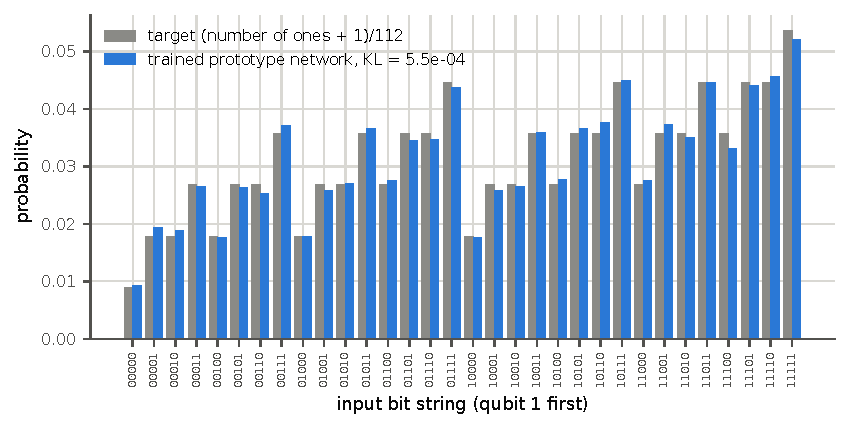
\includegraphics[width=\textwidth]{fig_bitcount_histograms}
\caption{Paper Fig.~5.  Target histogram (grey) and the trained prototype network's model
distribution (blue) over the 32 input strings.  Run \run{bitcount\_noise/20260820T145335Z}
(seed 1 of the bit-count training).}
\label{fig:histograms}
\end{figure}

\begin{figure}[t]
\centering
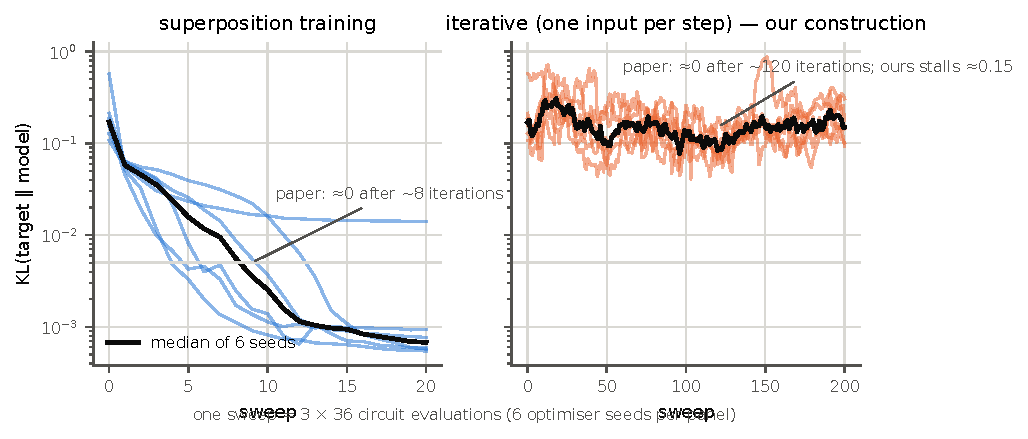
\includegraphics[width=\textwidth]{fig_bitcount_convergence}
\caption{Paper Fig.~6.  Left: superposition training, six seeds and their median.  Right:
our construction of the iterative baseline, which does not reach the paper's curve.  Run
\run{bitcount/20260820T135930Z}.}
\label{fig:convergence}
\end{figure}

\subsection{Iris: a dataset in superposition}
\label{sec:iris}

\paragraph{Task and encoding.}
Each of the four Iris features is quantised into three clusters by $k$-means, giving a 12-bit
one-hot code per flower; the whole training set is loaded as one superposition state over its
distinct codes, and the label is encoded in the amplitude.  The paper does not state how the
label enters; reading its Fig.~8 bar heights ($1/86, 4/86, 9/86$ on the training set and
$1/154, 4/154, 9/154$ on the test set, two independent integer normalisations) fixes the target
weight of class $\ell\in\{0,1,2\}$ to be proportional to $(\ell+1)^2$ --- the amplitude carries
$\ell+1$ and the histogram its square.  No other exponent produces both normalisations.  The
paper also does not state the train/test split; we use a stratified one-third training split
(50 flowers) and report the sensitivity.  The network has 12 inputs, 4 hidden neurons and one
output (17 qubits); a classic-neuron network of the same size is trained for comparison.
Predictions are made by reading each code's weight and rounding to the nearest label.

\paragraph{Result.}
\Cref{fig:iris-losses} is the paper's Fig.~7 on three data splits: the classic network drives
its training loss to $10^{-5}$ within a few sweeps while its test loss bottoms out early and
stays at $0.03$--$0.04$ (it memorises); the prototype network descends more slowly on both and
its test loss is still falling at sweep~40.  Test accuracy: $95\,\%$, $91\,\%$ and $98\,\%$ on
the three splits for the prototype network against a paper value of ``$\approx 98\,\%$''; the
encoding itself caps accuracy at $97\,\%$, $99\,\%$ and $99\,\%$ on those splits, because two
flowers of different species can share a 12-bit code.  \Cref{fig:iris-hist} is Fig.~8 for the
test split.  The Fig.~9 picture --- a two-dimensional embedding in which the prototype weights
are claimed to ``span the data'' --- does not reproduce: both weight sets cluster away from the
data in our embedding; we do not know what the authors plotted.

\paragraph{On the split.}
Fig.~8 shows 15 non-empty bars for the training set and 30 for the test set.  Our 50-flower
training splits produce 14, 12 and 14 distinct codes (close to 15), but the 100-flower test
splits produce only 20, 20 and 18 (not 30): a one-hot code with three clusters per feature does
not spread 100 flowers over 30 codes on any split we tried.  The figure therefore supports the
\emph{direction} of the split (test larger than train) but not its ratio, and the ratio remains
our assumption.

\begin{figure}[t]
\centering
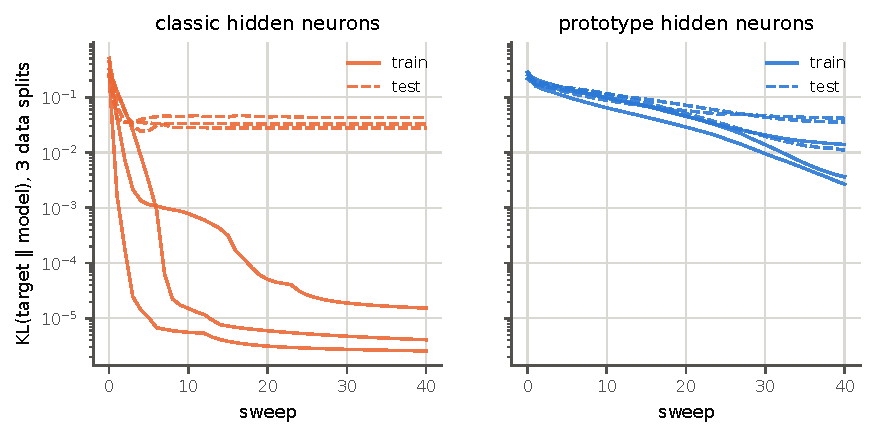
\includegraphics[width=\textwidth]{fig_iris_losses}
\caption{Paper Fig.~7.  Training (solid) and test (dashed) loss per sweep for three data splits.
Runs \run{iris/20260820T144849Z}, \run{…T145454Z}, \run{…T145455Z}.}
\label{fig:iris-losses}
\end{figure}

\begin{figure}[t]
\centering
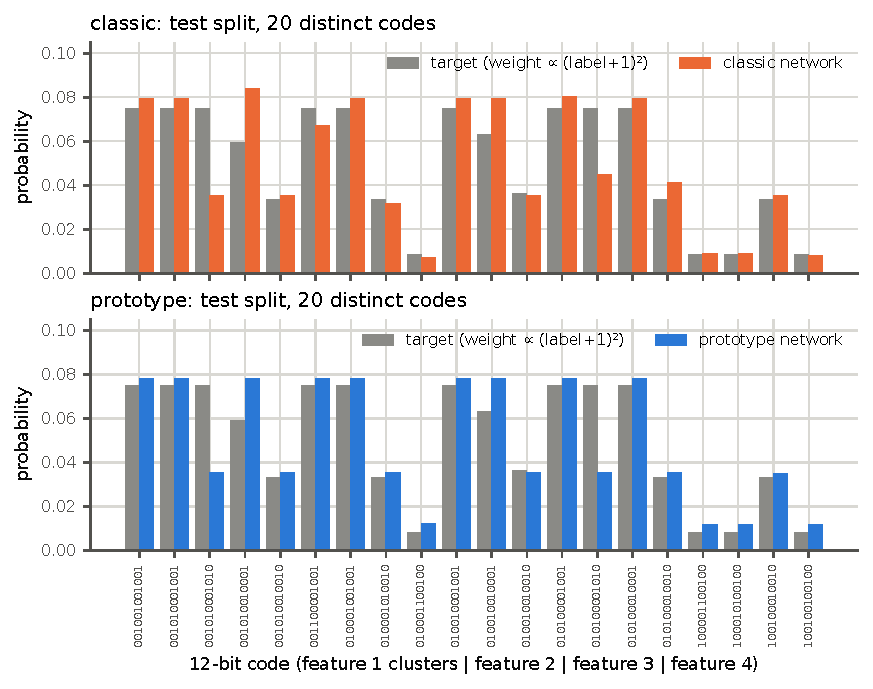
\includegraphics[width=\textwidth]{fig_iris_histograms}
\caption{Paper Fig.~8, test split of seed~0: target weight per distinct code (grey) against
the trained network's weight, classic (top) and prototype (bottom).  The bars are the
probabilities of reading each code together with the output firing, renormalised.}
\label{fig:iris-hist}
\end{figure}

\subsection{Flappy Bird: a seven-qubit controller}
\label{sec:flappy}

\paragraph{Task.}
Two features --- the bird's height and the centre of the next gap, both scaled to $[0,1]$ ---
enter two input qubits by \cref{eq:encoding}; four prototype hidden neurons and one classic
output decide ``flap'' when $\Pout > \tfrac12$ (paper, Fig.~10).  The paper says the trained
network ``plays the game perfectly'' and that a run was stopped after a score of 450\,000 that
took six days; it gives no reward, no training protocol and no game constants.  We built a
deterministic, window-free clone of the game.  Its physics are our choice: the classic
constants (flap impulse $-9$, gap 100, pipe spacing 144) are provably unplayable by a memoryless
policy on two features (one flap overshoots by 40.5 px against a 38 px budget), so we use impulse
$-7$, gap 120, spacing 180.  Training minimises the negative episode return (0.01 per frame
survived plus 1 per pipe) plus a small tracking term $|{\rm height} - {\rm gap}|$ that gives the
optimiser a slope in the region where every policy dies within 30 frames.  300 random parameter
vectors are scored on short episodes, the best seeds 25 sweeps of the optimiser on five
1500-frame training episodes.

\paragraph{Result.}
The trained network passes $110$ pipes in $5\,000$ frames --- the cap, i.e.\ a perfect game ---
on all 20 held-out game seeds, for all 8 optimiser seeds tried, in about three minutes of
training (run \run{flappy/20260820T143753Z}).  \Cref{fig:flappy-policy} shows what it learned: a
curved decision boundary in the (height, gap) plane, flapping when the bird is below the gap.  A
finding about the optimiser: rotating the five training episodes among a pool of ten every sweep
gave $0/25$ perfect games in the first session, and was recorded as a negative result; the cause
was that the optimiser kept its incumbent's loss from the previous batch, so every Metropolis
comparison compared scores on different games.  Re-scoring the incumbent on each new batch
restores $25/25$ perfect games (runs \run{flappy/batch0}, \run{flappy/batch5}), so the rotation
neither hurts nor helps here.

\begin{figure}[t]
\centering
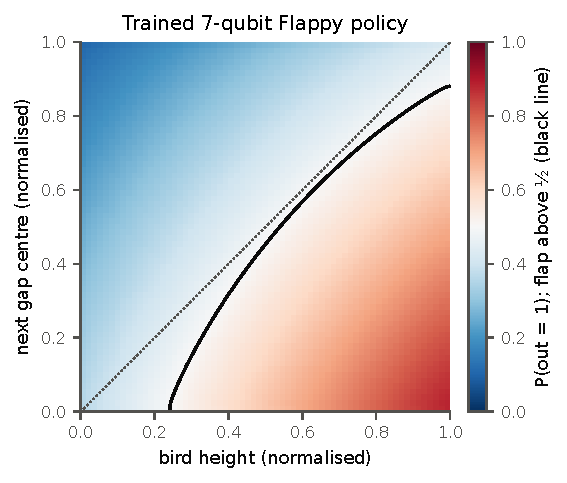
\includegraphics[width=0.5\textwidth]{fig_flappy_policy}
\caption{The trained Flappy controller's activation $\Pout$ over the two observations; the
black line is the decision boundary $\Pout = \tfrac12$ (flap to its right), the dotted diagonal
is ``bird at gap height''.  Run \run{flappy/20260820T143753Z}.}
\label{fig:flappy-policy}
\end{figure}

\subsection{ECG denoising}
\label{sec:ecg}

\paragraph{Task.}
A window of five consecutive noisy samples $s(t-2),\dots,s(t+2)$ enters five input qubits; one
to three prototype hidden neurons and one output predict the clean centre sample as $\Pout$
(paper, Fig.~12).  The paper does not say which recording it used; its Fig.~13 shows a smooth
two-beat trace of 1\,800 samples in $[0,1]$ with additive noise of standard deviation
$\approx 0.03$.  We generate a synthetic ECG of the McSharry form \cite{mcsharry} tuned to that
figure, add Gaussian noise of $\sigma = 0.02$ (noisy input $32.0$~dB), train on the first half and
test on the second, and repeat on PhysioNet MIT-BIH record~100 for comparison.  Quality is
measured by PSNR and SSIM (paper, Eqs.~(6)--(8)).

\paragraph{Result.}
\Cref{fig:ecg-trace} is the paper's Fig.~13; \cref{fig:ecg-table} is its Table~I.  We obtain
$37.4$, $38.0$ and $38.1$~dB for one, two and three prototype neurons against the paper's $32.9$,
$40.00$ and $40.04$: within about $2$~dB at two and three neurons, and $4$~dB \emph{above} the
paper at one neuron.  The prototype network beats the classic one at one and two neurons and on
every SSIM; the classic one wins at three.  Two notes.  The numbers cannot match exactly because
the signal is not the paper's; and the alternative angle encoding $\theta = \pi s$ costs
$0.6$--$7$~dB on this task, which is independent evidence for \cref{eq:encoding}.  On MIT-BIH
record~100 (run \run{ecg/20260820T165912}) the same networks reach $36$--$38$~dB.

\begin{figure}[t]
\centering
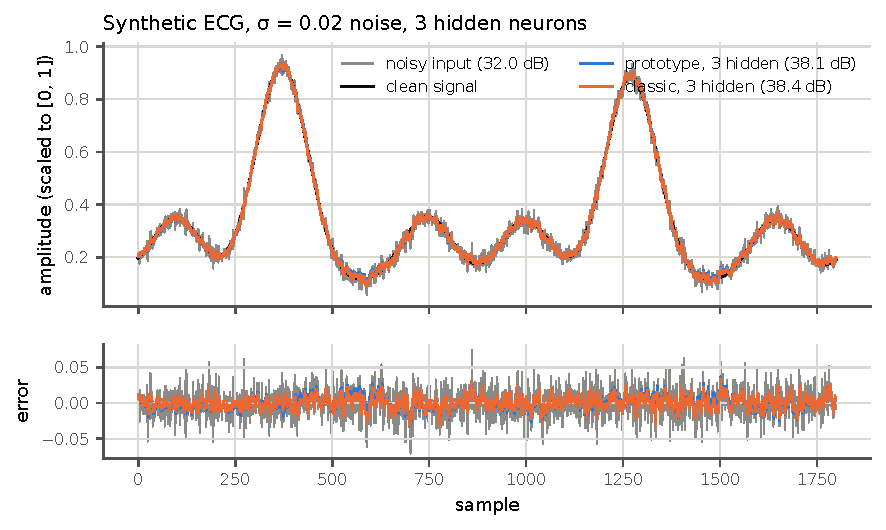
\includegraphics[width=\textwidth]{fig_ecg_trace}
\caption{Paper Fig.~13.  Noisy input, clean signal and the two three-neuron networks' outputs
(top); their errors (bottom).  Run \run{ecg/20260820T162014}.}
\label{fig:ecg-trace}
\end{figure}

\begin{figure}[t]
\centering
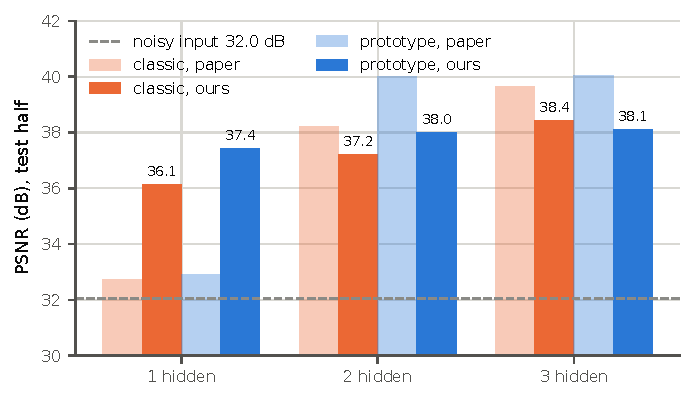
\includegraphics[width=0.7\textwidth]{fig_ecg_table}
\caption{Paper Table~I as a chart: PSNR on the test half for one to three hidden neurons,
paper values (light) against ours (dark).  Run \run{ecg/20260820T162014}.}
\label{fig:ecg-table}
\end{figure}
